%% Developing a solution for multimedia home networking chapter
%% author Liu Peng

To fulfill the need of interoperability among devices in home networking,
Tuxera Inc. started a project named Streambels(later renamed as AllConnect). The
project aims to solve the interoperability issue in multimedia home networking
by making a universal solution that can connect all available devices at home
and make them work together regardless of what protocol they use.\\
\\
Most devices at home are embedded solutions and have their own firmwares, it is
hard to update or even impossible to upgrade the software running on these
devices. On the other hand, most home network users
 are not knowledgeable enough to 
to manually set up the more advanced
 network features to achieve certain degree of device interoperability. Plus
 most of these network infrastructures are not designed to be easily
 configured. Due to these reasons, building interoperability among different
 devices through a mobile device seems to be the most straightforward solution,
 for mobile devices can serve as a very flexible and programmable portal for
 home-networking.  Other advantages of mobile devices include their great
 processing power, networking capabilities and their wide adoption and
 availability. Through the available platforms and tools, a mobile application
 could possibly be developed to control all multimedia streaming data flows and
 act as a personal access portal for home networking.\\
\\
After a year of development, our team have built up an Android application that
can be used to control and connect every known type of multimedia device at home.
Encouragingly, the number of our application users have grown to nearly one
million so far, providing a strong proof of the effectiveness of our solution.

\subsection{Architecture overview}
In order to solve the multimedia home networking interoperability problem, the system should be designed to control media playback sessions. Consequently, content navigation, manage receiver device, and media playback should be the most important three components. In our solution, the system architecture consists of three major parts: device discovery, content management and streaming.\\
\\
The discovery component is responsible for device discovery. As discussed
in\ref{upnp}, UPnP/DLNA devices and DIAL devices use Simple Service Discovery Protocol(SSDP) for device discovery. An application firstly sends a M-Search request over UDP to the IPv4 multicast address 239.255.255.250 and UDP port 1900. Then the application listens to other devices' responses. A DIAL device will return a response with an Application URL header, while the UPnP/DLNA devices will return a message with a XML body, which provides detailed service URLs and description URLs. Instead of using the SSDP discovery, Apple's products, in comparison, use Multicast DNS for device and service discovery. Obviously, in order to support the three types of devices, namely the UPnP/DLNA devices, the DIAL devices and the Apple Airplay devices, we need to integrate these two mentioned discovery mechanisms, namely, the SSDP mechanism and the Multicast DNS mechanism, into our solution.\\
\\
The content management component is responsible for organizing and
 navigating multimedia contents that can be discovered in the home network. In our solution, these content sources include both the local storage of smart phones and DLNA digital media servers that are connected to home network. As long as the discovered device belongs to the three device types that we support, its content could be streamed using our application solution.\\
\\
The streaming component is responsible for streaming multimedia content to the selected multimedia receivers, such as TVs, wireless speakers, set top boxes, etc. In a typical home networking environment, DLNA , AirPlay video/ photo and Chromecast all use HTTP streaming. The only exception, the AirPlay music, uses Remote Audio Output Protocol (RAOP). Because of this, we integrate two types of media servers inside our application solution. With our application, the built-in RAOP server would handle the AirPlay music streaming and the built-in HTTP media server would handle streaming of all other types.

\subsection{Implementation}
Since the application is built upon the Android platform, we conducted studies on the Android system architecture and the Android Software Development Kit (SDK). Thankfully, the Android SDK provides many useful Application Programming Interfaces (APIs) and grants crucial permissions to access necessary services and hardware features, such as the permission to access the Internet , the permission to access the WiFi device state change, the permission to allow WiFi multicast and  the permission to read phone storage. The programming language used in developing our Android Application is Java. However some CPU-intensive works, such as transcoding, have to be implemented in C and then embedded to the application using the Android Native development kit (NDK).\\
\\
Since Apple has not provided its official specification for AirPlay, our implementation for supporting AirPlay is mostly written under unofficial guidelines. However, Apple has provided its official Multicast DNS (mDNS) implementation. Thus, this piece of code is reused and compiled as a shared native library. Similar with the Airplay support, the support for Remote Audio Output Protocol (RAOP) is
 also implemented under unofficial guidelines. To be specific, the RAOP supporting component includes a UDP server and a TCP control channel.\\
\\
With Tuxera being a member of DLNA , we are able to access the detailed specifications and test tools for DLNA. Moreover,  there are a lot of open source UPnP/DLNA
 libraries available since DLNA is now a popular standard. Specifically, in our
 implementation, we uses a library called "cling"\cite{cling}, which provides minimal implementation of UPnP device discovery, description information parsing, and basic message handling. By extending "cling"\cite{cling}, we are able to provide media formats compatibility across different devices.\\
\\
Google has officially provided the Chromecast SDK for different mobile platforms, which enables us to  implement the Chromecast integration with ease. In the Streambels project, the Chromecast integration is built upon the Chromecast API.\\
\\
When it comes to media server implementation, according to the DLNA guideline,
certain additional headers need to be implemented in the stream. This
requires the HTTP server to possess the functionality to add DLNA specific
headers. Another requirement is that the "Seek" action needs to be supported on the server side. To support "Seek", byte based seeking operations are enabled in our implementation.\\
\\
For receivers who do not use the DLNA standard, a basic file server with byte range support will be sufficient to do the work.\\
\\
In order to serve media for all the receivers from both online and local storage, a separate media proxy also needs to be implemented.\\
\\
After investigating and comparing multiple server implementations on Android, we
concluded that NanoHTTPD is the ideal choice for our solution, because NanoHTTPD is easy to use,
Apache licensed, very tiny and efficient. Since NanoHTTPD is minimally implemented, it is easy to be modified and extended. With NanoHTTPD , additional headers can be easily added to make the server implementation compatible with DLNA receivers. Besides, a proxy is also easy to integrate with  NanoHTTPD.\\
\\
Taking all these technical details into consideration, we devised a simplified
architecture for our implementation, which is shown in Figure \ref{chart3}.
\begin{figure}[htb]
\centering 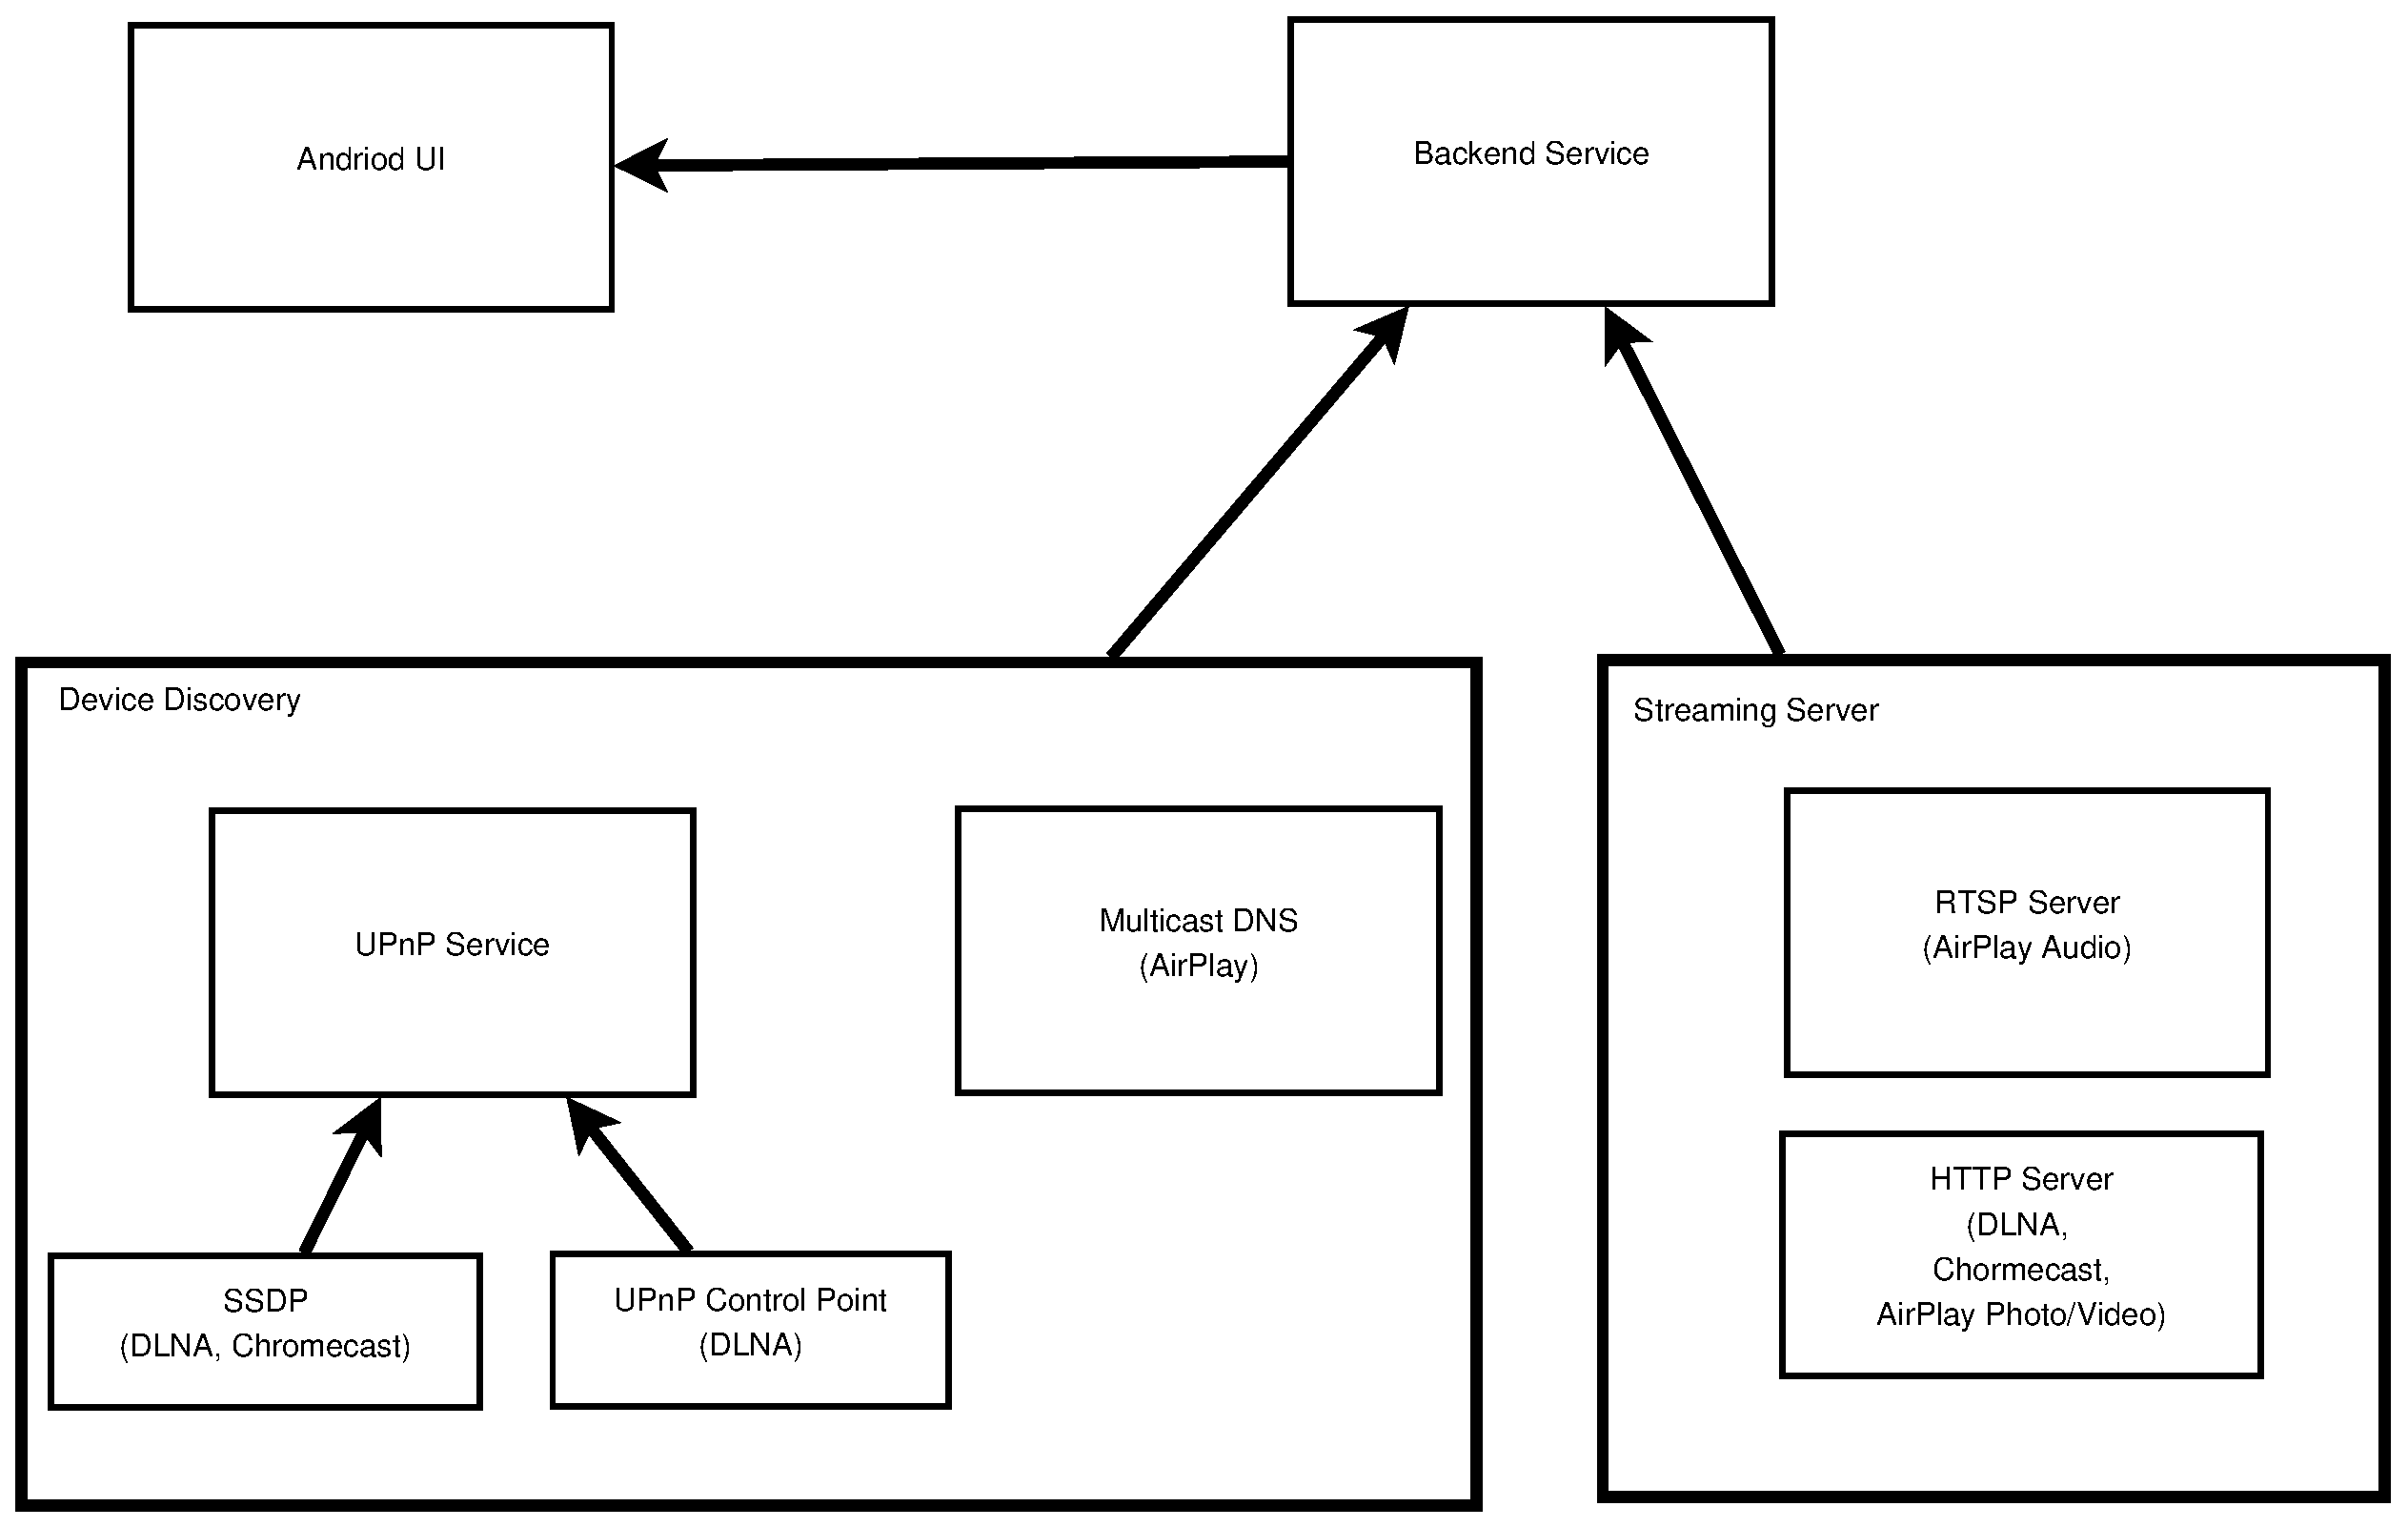
\includegraphics[height=9cm]{charts/chart3}
\caption{Simplified application architecture\label{chart3}}
\end{figure}\\
\\
When streaming content, the data flow is different for different scenarios. Figure \ref{chart4} shows the three use scenarios and their corresponding data flows:\\
\\ 
If the content is stored in a mobile phone, a streaming server in the application will be used to stream the content from phone to the selected receiver.\\
\\
In contrast, if the content is located on the Internet and the receiver is a DLNA Media Renderer, a proxy will be needed. To be specific, the proxy will first download the resource stream and then add certain headers required by the DLNA specification. After that, the proxy streams the modified content to the selected DLNA Media Renderer.\\
\\
Finally, if the streamed content locates in a DLNA Digital Media Server, then the source can be used directly by all receivers. In this case, the streaming proceeds directly from the media server to receivers. Our application, in this scenario, will only be used as a control point and do not really participate in the media transmission.\\
\\
\begin{figure}[htb]
\centering 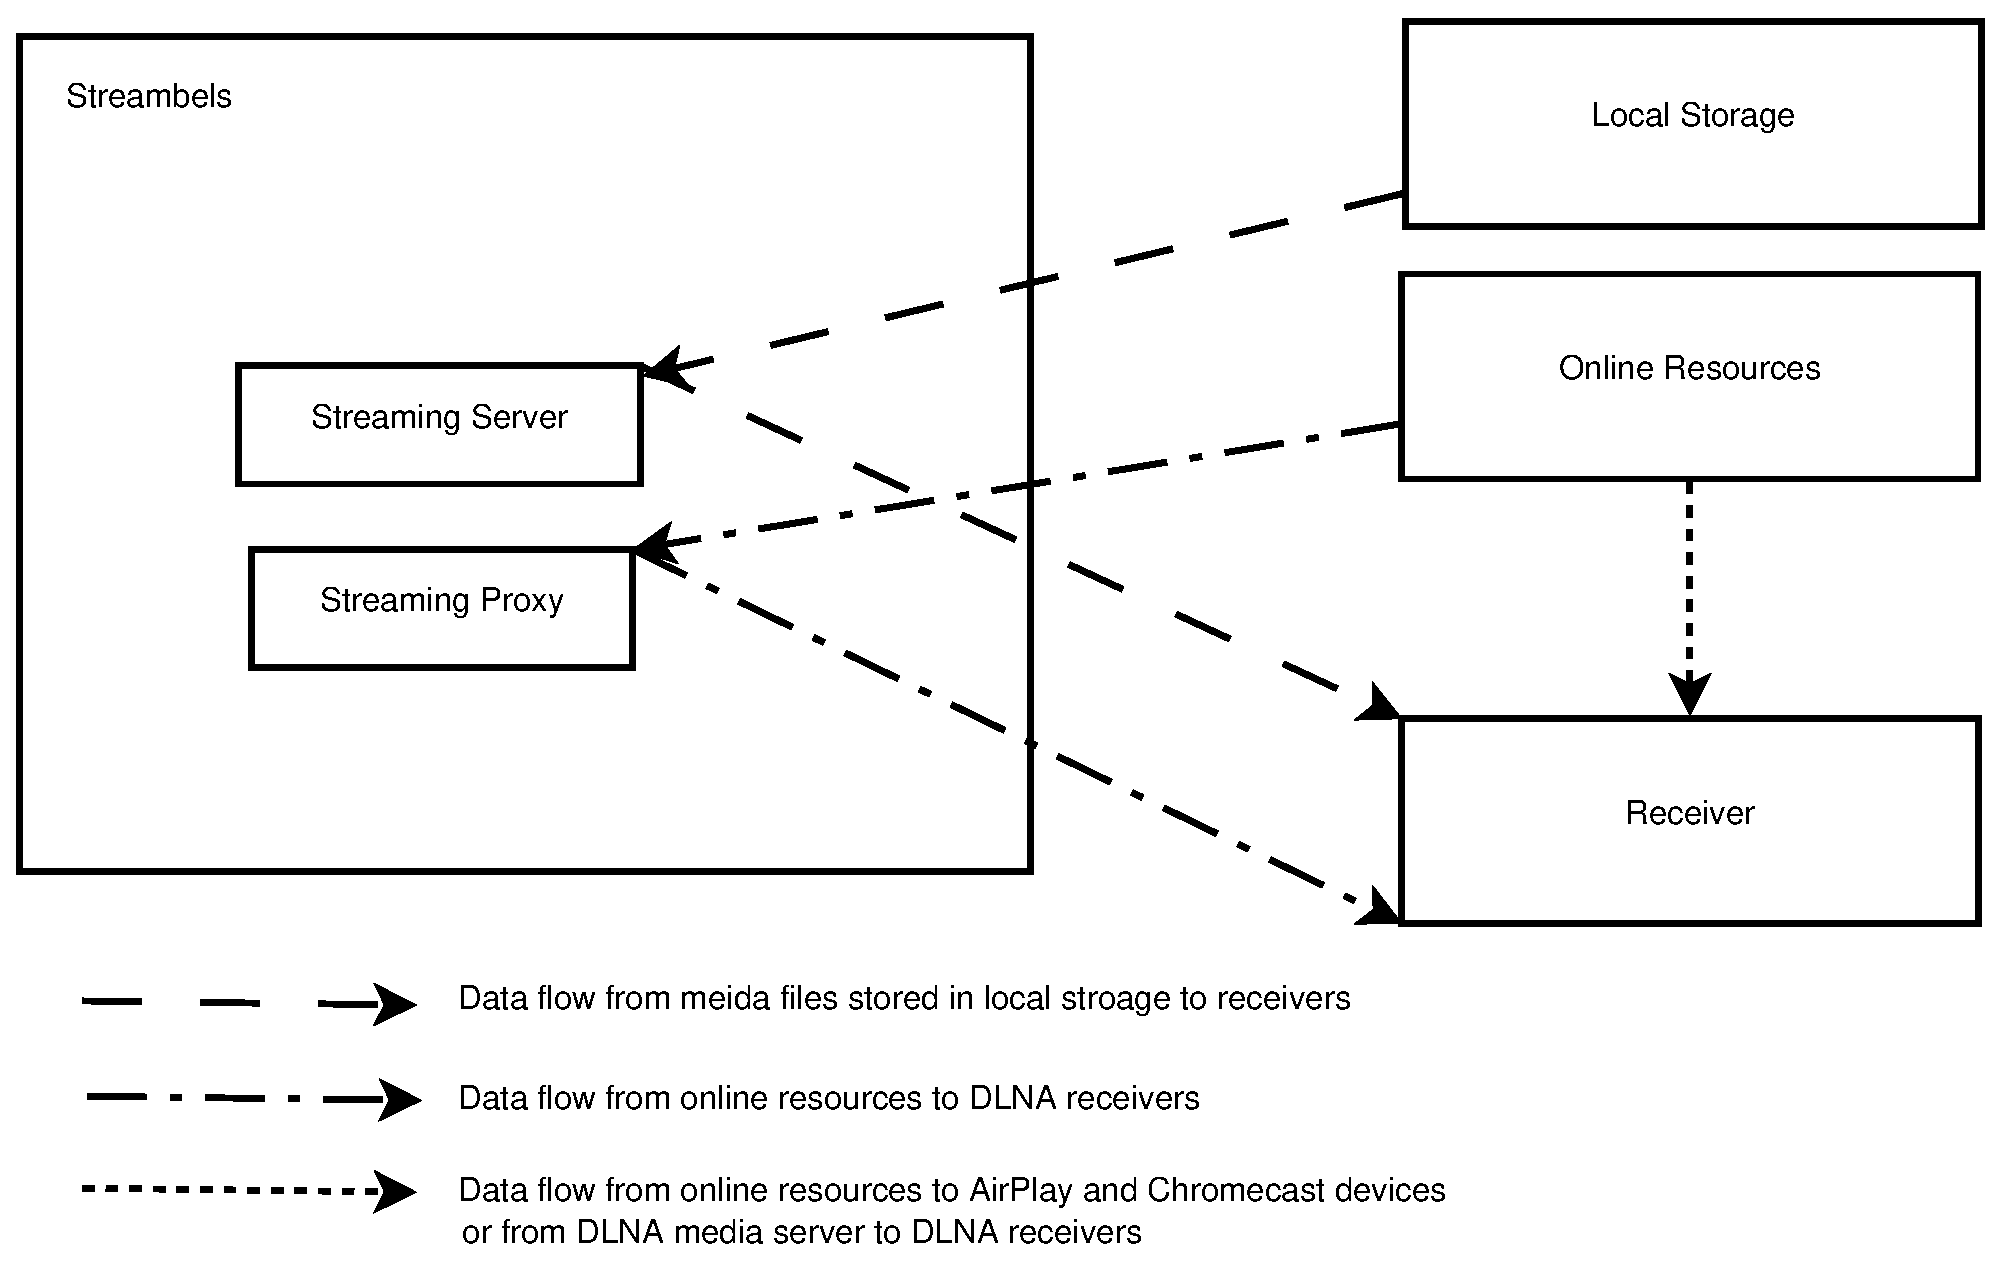
\includegraphics[height=9cm]{charts/data_flow}
\caption{Simplified data flow \label{chart4}}
\end{figure}

\subsection{UX design}
In terms of UI and UX, the application should be simple enough to use. Users should be able to locate the media, browse
 content on different sources, and follow the data flow between devices without any difficulty. The control of different devices should also be intuitive so that the inter-operation between different devices can be seamless.\\
\\
A multimedia home networking solution should be content centric so that user can easily navigate through different sources. The application is designed similar to a multimedia player. A cast button is added at the top of the application to make it easier to select cast devices. The content is categorized into 4 sections: music, video, photo and online sources. In Android, since the system provides share intent method for inter-activity communication, an interface is also made to manage share intents from other activities. The selected receiver is designed to be visible to user from everywhere inside the application. \\
\\
Bearing all these considerations in mind, the final appearance of the application becomes simple and effective. Figure \ref{chart5} shows the final design of our application.
\begin{figure}[htb]
\centering 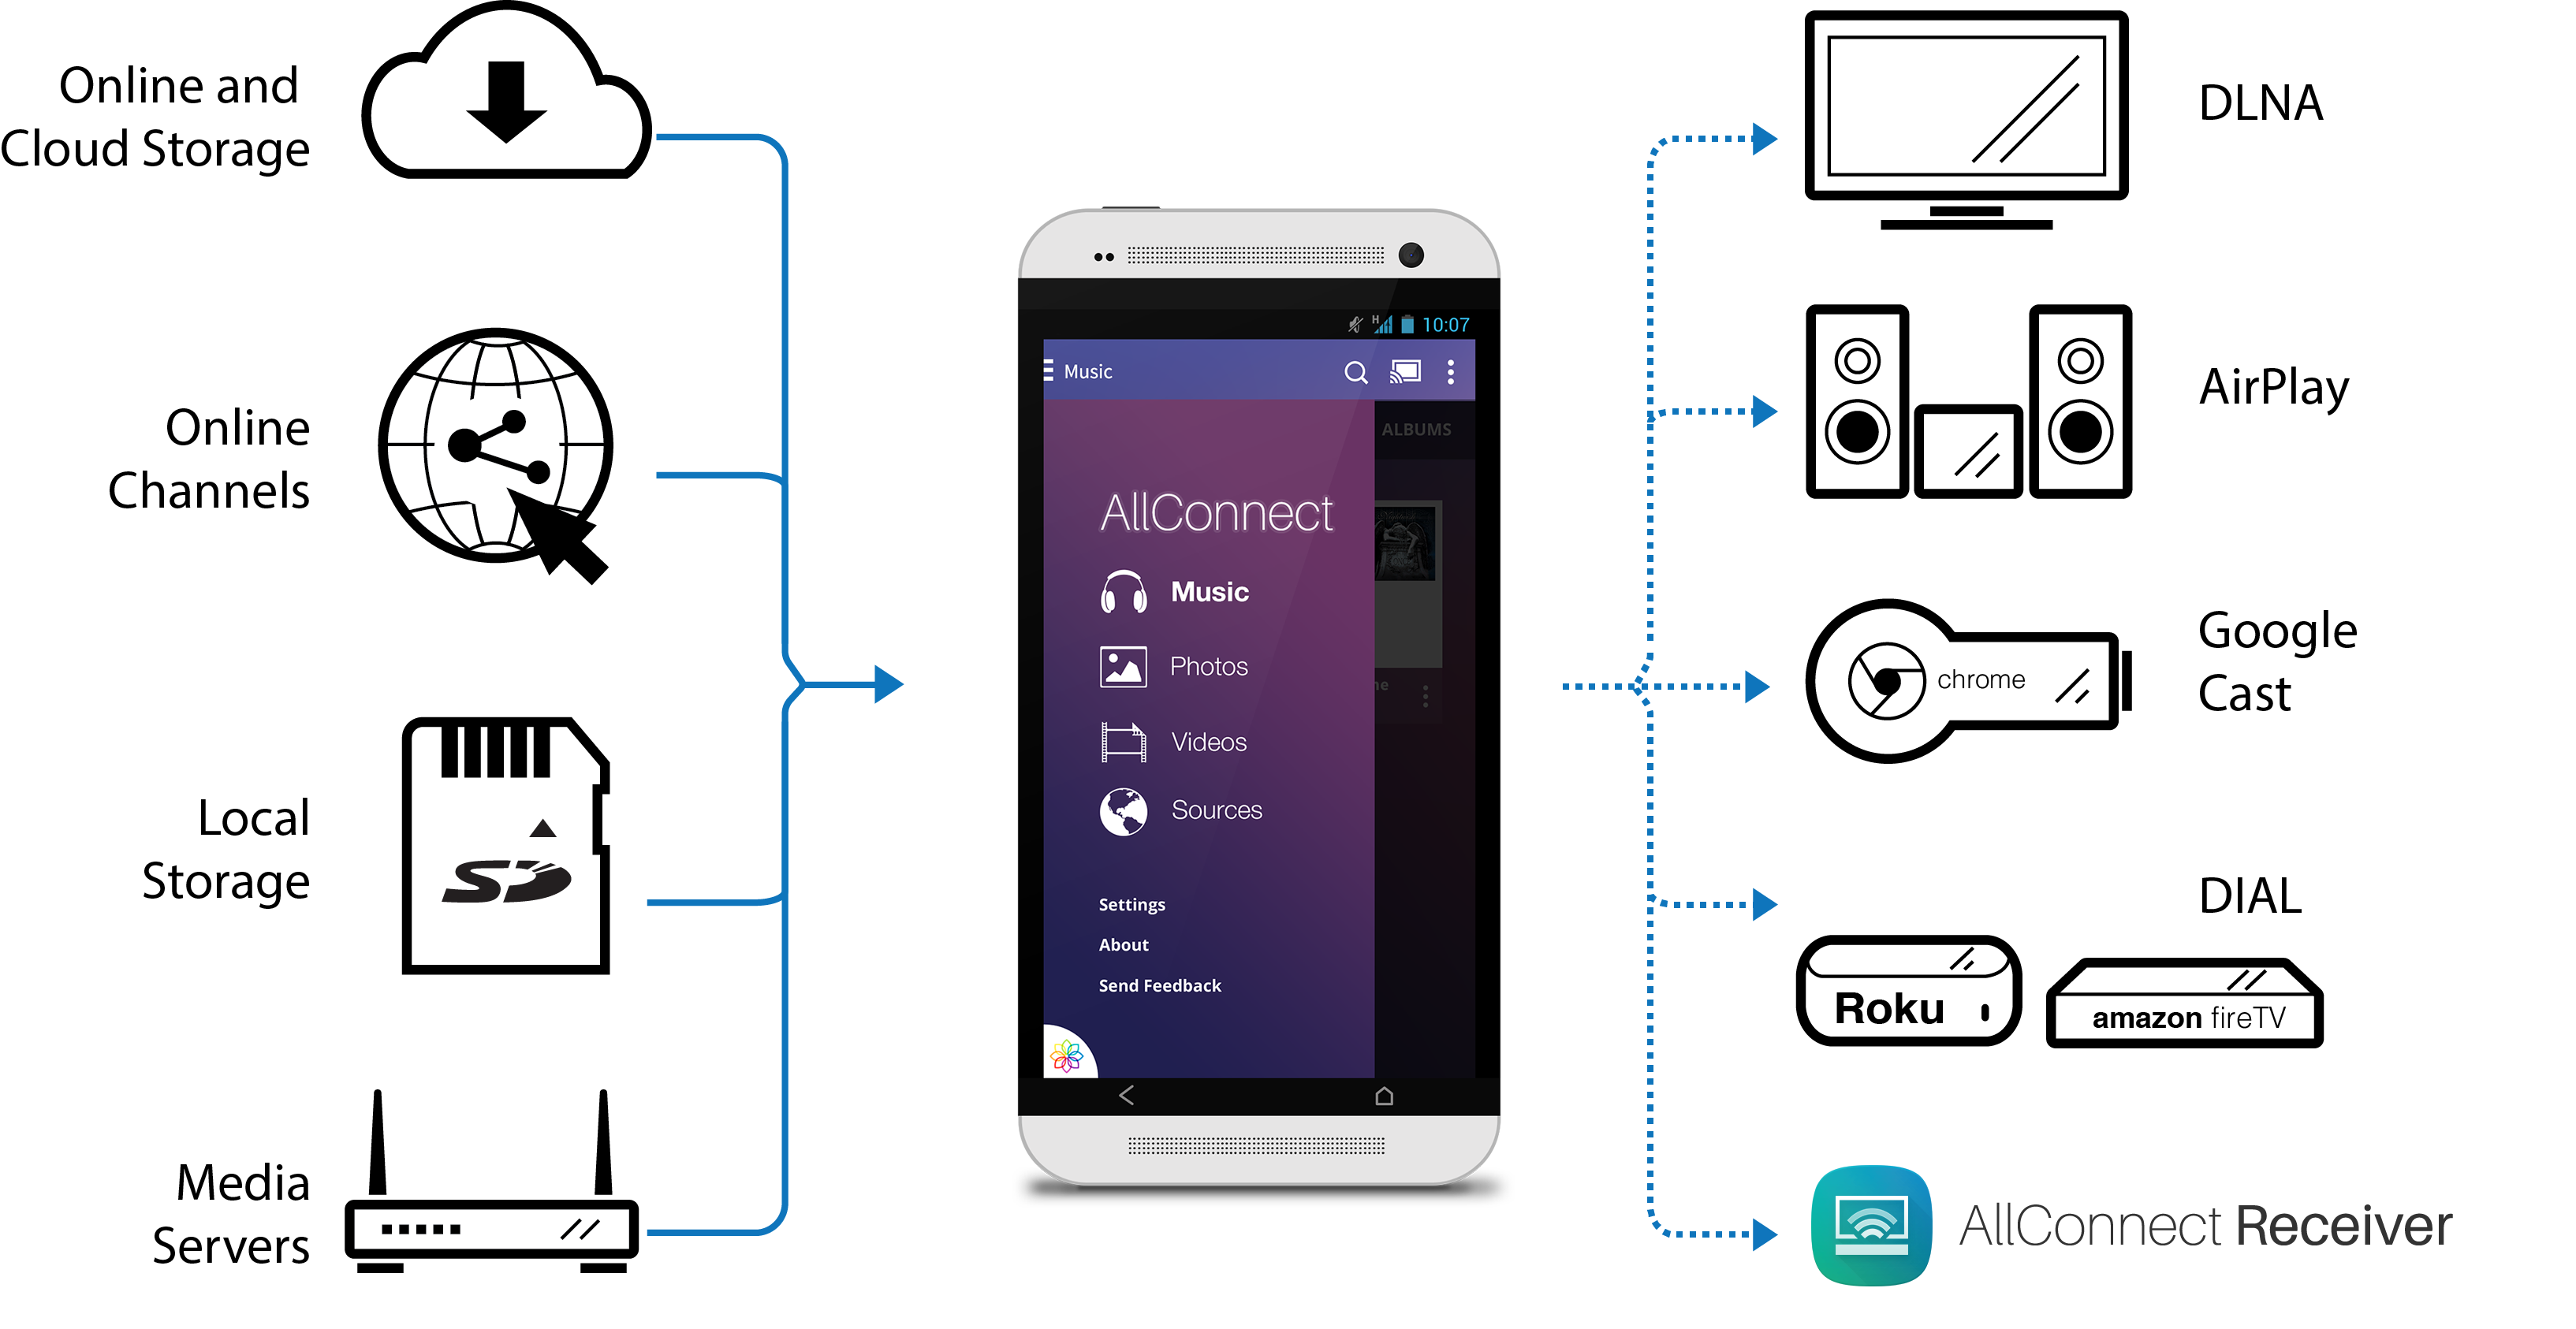
\includegraphics[height=8cm]{charts/allconnect-app}
\caption{Application UX design \label{chart5}}
\end{figure}

\subsection{Features}
The Android application we have developed can handle most multimedia devices in typical home networking. It also provides various features, making it a powerful and universal solution for multimedia home networking.\\
\\
Firstly, the application itself is a multimedia player. Both the media stored locally on the phone storage and the media located in the DLNA media servers can be browsed and played locally on the phone.\\
\\
Secondly, the application is fully compatible with AirPlay, DLNA, Chromecast and FireTV receiver devices. All devices can be discovered as renderer devices.\\
\\ 
Thirdly and most importantly, the application enables the DLNA media server to work together with all kind of receivers regardless of the protocol used. The app served as a bridge for different multimedia receivers and media sources.\\
\\
Lastly, YouTube and other on-line channels like Vimeo and Facebook are supported as available media sources. These content can be streamed, regardless of the protocol, to all supported receivers that are connected to home network.

\subsection{Extensibility}
Streambels has embedded a media streaming server for local files and a streaming proxy for bridging the gap between online resources and home networking. By using a built-in proxy, Streambels is able to share on-line resources from the Internet to devices in home networking environment. \\
\\
New service providers and content providers can integrate home networking support into their products easily by just sending formatted intent to our application following our guidelines. The proxy will automatically bridge the gap between the Internet and home network.\\
\\
The proxy system provides great extensibility and makes it possible to connect home networking to Internet or Cloud Services.\\
\\
In the future we could also develop a Software Development Kit (SDK) to grant the availability of our technology, enabling other application builders to directly use our home-networking solutions.
\subsection{Test methodology}
Software testing is extremely important for a modern IT project. Buggy implementations may kill the product in the very beginning since it can badly undermine user experiences. Through testing we could assure the performance and stability of our product. Thus, before the final releasing to the Google Play store, the application was thoroughly tested.\\
\\
These tests included unit test, integration test and functional test.
Unit tests were conducted while coding the application. When each class was finished, unit tests would be written for each method. We also set up an continuous integration server so that each time we commit anything to the git repository, full set of unit tests would be executed. If there were any failure in the unit tests, developer would be immediately notified. Integration tests were done in such a way that we ensured each function module work together with other modules in the system. Lastly, we listed all the possible use cases in paper and prepare a huge media base which contains all kind of media files. With all these preparations ready, manual tests were conducted before the app is finally released in the market.

\subsection{Evaluation methodology}
The evaluation of this application includes two parts. The first part involves experiment
s
that help evaluate the application performance. The second part invovles a study on the application usage in the market and user feedbacks.

\subsubsection{Experimental setup}
The test environment is set up as in Figure \ref{}. The XBMC media receiver is running on MacBook A and Streambels is running on a rooted Android phone. Both A and B are connected to a router C using the 802.11 g wireless interface. \\
\\
With the support of both AirPlay and DLNA protocols, XBMC is an open source media center software that can run on different platforms. It is a popular software solution that is widely used in home networks, which has been ported to different platforms including Raspberry PI.\\
\\
Network Link Conditioner is an application provided by Xcode that runs on Mac to emulate network conditions, such as packet loss, network delay and bandwidth variations. By changing the configurations, different network conditions can be set to determine the boundary network conditions.\\
\\
Wireshark is an useful developer tool to capture and analyze network traffic. It can be installed on both the sender and receiver side. However, it can only be installed on rooted Android phones to gain the access to network interface on Android. In our setup, Wireshark is installed on MacBook because we need to adjust network condition on the receiver side and there might be packet loss since some protocols may use UDP protocol.\\
\\
When the test starts, the same content will be streamed to receivers using two different standards, AirPlay and DLNA. The same test will be run several times to get the average statistics. Different parameters will also be tested by using different network condition configurations.
\\
3 parameters are taken into consideration when conducting the tests: bandwidth, packet loss and delay. 
\subsubsection{User study and feedback collection}
Since the product is targeted to Android market and is directly used by end users, user feedback is really important to us for improving the product continuously. Email is used for normal communication between user and our support. A submission window is built inside the application, so that users can easily send feedback to us directly by Email.\\
\\
There is no perfect program, crashes sometimes happen. Thanks to Google, all crash reports are collected and displayed inside developer console. This makes it a lot easier to track and debug our application.\\
\\
Inside Streambels, we also integrated Google's Analytics API. The API provided great convenience for us to collect number of users and sessions every day. Other information such as operating system version, application version and the number of active users as well as user feedbacks, have helped us to gain more insight in our application and the market response, making it easier for us to improve the application and do better marketing. 
\\
It is also interesting to see what kind of technologies are most used in their daily life. With the analytics SDK, we could trigger events when user select their receivers. After months of monitoring and statistics collection, we have been able to figure out the most popular standards and most popular online channels .\\
\\
These valuable information will in turn help our decision making on how we should improve our application. Some of these result will be discussed in chapter 4.
